\documentclass[conference]{IEEEtran}
\IEEEoverridecommandlockouts

\usepackage{cite}
\usepackage{amsmath,amssymb,amsfonts}
\usepackage{algorithmic}
\usepackage{graphicx}
\usepackage{textcomp}
\usepackage{xcolor}
\usepackage{booktabs}
\usepackage{url}

\def\BibTeX{{\rm B\kern-.05em{\sc i\kern-.025em b}\kern-.08em
    T\kern-.1667em\lower.7ex\hbox{E}\kern-.125emX}}

\graphicspath{{figures/}}

\begin{document}

\title{AquaScan: An Offline-First Mobile System for Freshwater
Fish Disease Classification with Uncertainty Gating and
Retrieval-Grounded Assistance}

\author{
\IEEEauthorblockN{Rachit Bhusal}
\IEEEauthorblockA{\textit{Computing Sciences Division} \\
\textit{Arkansas Tech University}\\ Russellville, AR, USA \\
rachitbhusal@gmail.com}
\and
\IEEEauthorblockN{Robin Ghosh}
\IEEEauthorblockA{\textit{Dept. of Engineering and Computing Sciences} \\
\textit{Arkansas Tech University}\\ Russellville, AR, USA \\
rghosh@atu.edu}
}

\maketitle

\begin{abstract}
Fish disease is still judged at the pond edge by eye, and a wrong call costs stock and time. We describe AquaScan, a working system that turns a seven-class freshwater fish disease classifier into something a farmer can actually use, and we are careful to separate what we measured from what we did not. The classifier is a 2.20-million-parameter convolutional network trained on the public South Asian freshwater fish disease corpus, with one preprocessing routine shared byte-for-byte by training, evaluation, and serving. On the distributed \texttt{Test/} directory it reaches 81.29\% top-1 and 95.14\% top-3 accuracy at a macro $F_1$ of 0.812 (95\% bootstrap CI $[0.782,0.840]$), beating an earlier checkpoint by 11.86 accuracy points; because per-image logs were lost we cannot run McNemar's test exactly, but the marginals alone bound it at $p \leq 7.9\times10^{-6}$. We then audited the corpus, and the result reframes that headline. All 700 images in \texttt{Test/} are byte-identical copies of images in \texttt{Train/}, so the nominal 2\,450-file dataset holds 1\,747 distinct photographs and any score on that directory measures recall of fitted data. The 63.71\% we obtain on an internal held-out split is the only generalisation estimate this study can defend. Around the classifier sit an ImageNet fish-presence gate, a joint confidence--entropy rejection rule, and a retrieval-augmented assistant that answers follow-up questions from a local 36-chunk aquaculture index through a quantised on-device language model, with retrieval conditioned on the prediction. Baseline comparisons, gate accuracy, and retrieval quality are given as protocols and reported as outstanding, not estimated.
\end{abstract}

\begin{IEEEkeywords}
fish disease classification, convolutional neural networks, aquaculture, dataset duplication, out-of-distribution rejection, retrieval-augmented generation, uncertainty estimation, mobile deployment
\end{IEEEkeywords}

% =========================================================
% I. INTRODUCTION
% =========================================================
\section{Introduction}

Inland aquaculture supplies a large share of the animal protein eaten in South Asia, and disease outbreaks are among the most damaging shocks that supply absorbs year after year \cite{b33}. The warning signs are visible long before a laboratory can confirm anything: haemorrhagic patches, eroded fins, inflamed gills, fungal growth, white caudal lesions. They are also easy to mix up. A farmer who reads a parasitic infestation as a bacterial one loses the treatment window and pays for the wrong intervention on top of it.

Convolutional networks suit this decision well. Working on a seven-class South Asian freshwater corpus, Tamut \emph{et al.} \cite{b1} showed that a compact three-block network separates the categories, reporting 99.71\% accuracy at a test loss of 0.0119. That tells us the visual problem is learnable, and it gives us an architecture to start from. It tells us nothing about what a farmer holding a phone will actually experience.

Three gaps sit between that benchmark and a usable tool. The first is \emph{evidential}. A classifier is worth only as much as the split it was scored on, and the audit in Section~\ref{sec:model} finds that the public corpus contains no test image that is not already in its training directory. The second is \emph{behavioural}. A seven-way softmax is a closed set: photograph a bucket and it will still name a disease. Section~\ref{sec:app} describes the two-stage service that catches those inputs before the classifier sees them. The third is \emph{interpretive}. A label and a percentage do not tell anyone what to do next, and a general-purpose chatbot will answer the follow-up from parametric memory with nothing to check it against. Section~\ref{sec:llm} describes an assistant that answers from a curated index plus the current prediction, runs on the operator's own machine, and shows the passages it used.

We contribute five things. A duplicate-aware re-reading of a widely used public corpus, with the audit that supports it. A classifier trained under a single shared preprocessing contract and reported with bootstrap and Wilson intervals, a full confusion analysis, and a distribution-free significance bound against an earlier checkpoint. A deployed two-stage service and cross-platform client in which gating, rejection, and confidence tiering are visible parts of the product rather than internal details. A fully local retrieval-augmented assistant whose retrieval query is conditioned on the classifier output. And, throughout, a clean line between what we measured and what still needs doing. Fig.~\ref{fig:system} shows how the pieces connect.

\begin{figure*}[!t]
\centering
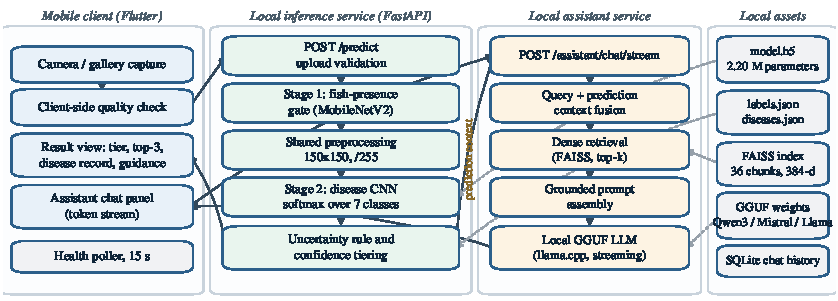
\includegraphics[width=0.74\textwidth]{fig_system.pdf}
\caption{AquaScan system architecture. The assistant path reuses the classifier output as retrieval context, and every model and data asset resides on the operator's machine.}
\label{fig:system}
\end{figure*}

% =========================================================
% II. RELATED WORK
% =========================================================
\section{Related Work}

Reported accuracies for image-based fish health assessment span a very wide band, mostly because dataset size, class definition, and split policy differ from paper to paper. Tamut \emph{et al.} \cite{b1} trained a three-block network from scratch on the seven categories used here for 50 epochs at batch size 32 with Adam \cite{b12}, reporting 99.71\% accuracy, and also report a ResNet50 \cite{b8} transfer trial reaching only 70.83\% validation accuracy; they identify bacterial gill and bacterial red disease as the pair most often confused, an observation Section~\ref{subsec:error} revisits. Ahmed \emph{et al.} \cite{b38} compared four backbones on Bangladeshi aquaculture imagery and reported 82.51\% test against 95.51\% validation accuracy --- a gap that is itself an argument for reporting held-out figures --- and Biswas \emph{et al.} \cite{b39} evaluated transfer-learning and fusion approaches on the same problem. Every one of these figures rests on the same assumption: that the evaluation images were not seen during fitting. The assumption fails quietly and it fails often. Near-duplicates across the CIFAR splits inflate apparent accuracy \cite{b34}, standard corpora carry large-scale semantic redundancy \cite{b35}, and test-set defects have been shown to reorder model rankings outright \cite{b36}. Checking for duplication is a precondition for evaluation, not an appendix to it.

Two further literatures shape the deployed system. A softmax cannot express ``none of these''; maximum softmax probability is the baseline out-of-distribution detector \cite{b25}, Shannon entropy \cite{b24} supplies a complementary uncertainty measure, and modern networks are systematically overconfident \cite{b23}. Separately, retrieval-augmented generation \cite{b4} conditions a language model on passages fetched at inference time, making an answer's sources inspectable and the knowledge base correctable without retraining; practical systems pair a sentence encoder \cite{b5}, \cite{b37} with a vector index \cite{b6}, and retrieval quality, grounding, and hallucination rate require separate measurement \cite{b40}, \cite{b41}.

% =========================================================
% III. MODEL DEVELOPMENT
% =========================================================
\section{Model Development}
\label{sec:model}

\subsection{Dataset and Content Audit}
\label{subsec:dataset}

AquaScan is trained on the public ``Freshwater Fish Disease Aquaculture in South Asia'' corpus \cite{b2}, distributed as \texttt{Train/} and \texttt{Test/} directories with one subdirectory per class: bacterial red disease, bacterial aeromoniasis, bacterial gill disease, fungal saprolegniasis, healthy fish, parasitic disease, and viral white tail disease. The class-to-index mapping is pinned in a version-controlled \texttt{labels.json} read by training, evaluation, and serving alike, and the service refuses to start if the loaded network's output width disagrees with it, removing an entire class of silent label-permutation faults. Counting files gives 2\,450 readable images: 1\,750 in \texttt{Train/} at 250 per class, 700 in \texttt{Test/} at 100 per class, a class-imbalance ratio of 1.00, and nothing unreadable. Before trusting that split we audited its contents, hashing every image twice --- SHA-256 over the raw bytes, and a 64-bit difference hash over an EXIF-corrected $9\times8$ greyscale reduction.

The result (Table~\ref{tab:audit}) left little room for interpretation. There are 698 exact duplicate groups. Every one of them crosses the train/test boundary, and all 700 files in \texttt{Test/} belong to one. Put plainly: the distributed test directory contains no image that is not already sitting in the training directory, byte for byte. Collapse the groups and 1\,747 distinct photographs remain, meaning 703 of the 2\,450 files are copies. Duplication \emph{inside} \texttt{Train/} is a different story --- three groups covering six images --- so the internal validation split described in Section~\ref{subsec:preproc} is essentially clean. Beyond the exact matches, 208 cross-split pairs agree at Hamming distance $\leq 4$ without being byte-identical, covering 181 distinct test images. One exact group and five near-duplicate pairs carry contradictory labels; in the exact case the same photograph is filed under both \emph{bacterial gill disease} and \emph{parasitic disease}.

\begin{table}[!t]
\caption{Content Audit of the Distributed Corpus}
\label{tab:audit}
\centering
\footnotesize
\begin{tabular}{lr}
\toprule
\textbf{Property} & \textbf{Value}\\
\midrule
Readable files (\texttt{Train/} 1\,750, \texttt{Test/} 700) & 2\,450\\
Unreadable files / train imbalance ratio & 0 / 1.00\\
Exact (SHA-256) duplicate groups, all cross-split & 698\\
\texttt{Test/} files with a byte-identical \texttt{Train/} twin & 700 / 700\\
Groups containing $\geq 2$ \texttt{Train/} files & 3\\
\textbf{Distinct images after collapsing duplicates} & \textbf{1\,747}\\
Cross-split near-duplicate pairs (Hamming $\leq 4$) & 208\\
\quad distinct \texttt{Test/} images involved & 181\\
Duplicate groups / pairs with label conflicts & 1 / 5\\
\bottomrule
\end{tabular}
\end{table}

This cuts the same way for us as for everyone else who has used this corpus. A model fitted on \texttt{Train/} has already seen every image in \texttt{Test/}, so a score on that directory measures how faithfully the model reproduces labels for photographs it was fitted on. It says nothing about new fish, new farms, or new cameras. We still report those numbers in Section~\ref{subsec:eval}, for two reasons: they are what the deployed artefact actually produces, and they are the only figures comparable with published work. But we label them in-sample every time they appear.

\subsection{Preprocessing, Architecture, and Training}
\label{subsec:preproc}

Preprocessing lives in one module, called identically by the training data loader, the offline evaluator, and the request handler. This is not tidiness for its own sake: a mismatch between the fitting path and the serving path cost us more accuracy during development than any modelling decision, and centralising the transform is the structural fix rather than a workaround. The pipeline applies the EXIF orientation transform, converts to three-channel RGB, resizes to $150\times150$ with Lanczos resampling, and scales to $[0,1]$; images whose short side falls below 64 pixels are flagged rather than refused. Augmentation runs only during training and only \emph{after} the shared transform, so it can never become a hidden difference between fitting and serving: horizontal flip, rotation to $\pm30^{\circ}$ with reflection fill, translation to 15\% of each axis, zoom within $\pm20\%$, and contrast and brightness jitter of $\pm20\%$. Vertical flips and hue shifts are excluded because fish orientation and lesion colour carry class information.


The deployed network follows the three-block design of \cite{b1}, adopted because it is validated on this exact taxonomy and because 2.20\,M parameters keep the serialised weights small enough to ship offline. Its structure, recovered from the serialised artefact rather than from documentation, is Conv2D($5\times5$, 128) $\rightarrow$ Conv2D($3\times3$, 64) $\rightarrow$ Conv2D($3\times3$, 32), each followed by $2\times2$ max-pooling, batch normalisation \cite{b28}, and 25\% dropout \cite{b27}, then Flatten(8\,192) $\rightarrow$ Dense(256, ReLU) $\rightarrow$ Dropout(0.5) $\rightarrow$ Dense(7, softmax), with an L2 penalty of $10^{-4}$ on every kernel; the total is 2\,202\,087 parameters, of which 2\,201\,639 are trainable. Three things about this design are worth flagging, because they are what Section~\ref{subsec:baselines} is really testing. Feature width \emph{decreases} with depth, which is the reverse of the usual convention; the wide $5\times5$ first layer suits the coarse, high-contrast lesion patterns that separate these classes, and narrowing the later blocks keeps the $73\times73\times128$ intermediate map affordable. With fewer than 1\,500 effective training images, the regularisation density is not optional. And the parameter budget is lopsided: the 256-unit layer after flattening alone carries 2\,097\,408 parameters, 95.2\% of the model, where global average pooling would need 8\,448. Most of this network is one fully connected layer.

Training holds out 15\% of \texttt{Train/} per class under a fixed seed of 42 and never touches \texttt{Test/}. The deployed checkpoint used batch size 32 over 60 epochs at an initial learning rate of $8\times10^{-4}$, AdamW \cite{b11}, and categorical cross-entropy with label smoothing 0.05 \cite{b29} on Keras 3.14; early stopping monitored validation loss with patience 15 and restored the best weights, and the learning rate was halved on plateau with patience 5, falling four times to $5\times10^{-5}$. Label smoothing was introduced because the raw network was confidently wrong on ambiguous bacterial cases, a direct usability problem for a tool that displays a confidence percentage; AdamW decouples weight decay from the adaptive step, although the deployed checkpoint predates the change that disables kernel L2 when AdamW is active and therefore carries both; and class weights use the effective-number formulation \cite{b3}, which on this balanced corpus evaluates to 0.998 for six classes and 1.012 for the seventh and is retained for the imbalanced field data anticipated in Section~\ref{sec:future}. Both callbacks monitor loss rather than accuracy, because under label smoothing the loss is the more sensitive indicator of when calibration stops improving.

Best internal validation accuracy is 63.71\% at epoch 51, with the minimum validation loss of 1.3010 arriving at epoch 56 (Fig.~\ref{fig:training}). That sits well below the 81.29\% we get on the distributed test directory, and at first glance it looks like something is broken. The audit explains it. The validation split holds images the network never saw; the test directory holds images it saw repeatedly. We therefore treat 63.71\% as the generalisation estimate this study can support, and 81.29\% as a reproduction measure. The gap between the two curves, opening under augmentation and dropout that are already aggressive, points at training-set diversity rather than model capacity as the thing holding this model back.

\begin{figure}[!t]
\centering
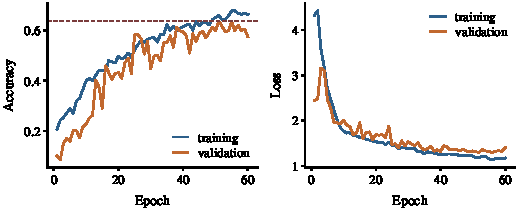
\includegraphics[width=\columnwidth]{fig_training.pdf}
\caption{Training and validation trajectories over 60 epochs. The dashed line marks the best validation accuracy, 63.71\% at epoch 51; the restored checkpoint is the one minimising validation loss at epoch 56.}
\label{fig:training}
\end{figure}

\subsection{Evaluation and Comparison Against a Previous Checkpoint}
\label{subsec:eval}

The offline evaluator loads the model through the same loader the service uses, applies the shared transform, and predicts over all 700 images. Table~\ref{tab:results} collects the results. Aggregate intervals come from 10\,000 bootstrap resamples \cite{b19}, and we cross-checked the accuracy interval with the Wilson score method \cite{b17}; the two agree to within three thousandths. Class supports are exactly equal here, so macro and weighted averages coincide and balanced accuracy equals top-1 accuracy. The most useful number in the table is the 13.9-point gap between top-3 and top-1: in 95.14\% of cases the correct condition is somewhere in the three-item differential the interface shows, even when the top-ranked label is wrong. That gap is the reason the interface never displays a bare verdict.

\begin{table}[!t]
\caption{In-Sample Performance on the Distributed \texttt{Test/} Directory
($N=700$; Per-Class $n=100$)}
\label{tab:results}
\centering
\scriptsize
\setlength{\tabcolsep}{4pt}
\begin{tabular}{lccc}
\toprule
\multicolumn{4}{c}{\textit{Aggregate metrics with 95\% intervals}}\\
\midrule
Top-1 accuracy (bootstrap) & \multicolumn{2}{c}{0.8129} & $[0.7829, 0.8414]$\\
Top-1 accuracy (Wilson) & \multicolumn{2}{c}{0.8129} & $[0.7823, 0.8400]$\\
Top-3 accuracy & \multicolumn{2}{c}{0.9514} & ---\\
Macro precision & \multicolumn{2}{c}{0.8223} & $[0.7938, 0.8494]$\\
Macro recall / balanced acc. & \multicolumn{2}{c}{0.8129} & $[0.7839, 0.8406]$\\
Macro $F_1$ & \multicolumn{2}{c}{0.8125} & $[0.7820, 0.8397]$\\
Matthews correlation \cite{b21} & \multicolumn{2}{c}{0.7834} & $[0.7498, 0.8160]$\\
Cohen's $\kappa$ \cite{b20} & \multicolumn{2}{c}{0.7817} & $[0.7469, 0.8146]$\\
Log loss & \multicolumn{2}{c}{0.7830} & ---\\
\midrule
\multicolumn{4}{c}{\textit{Per-class results, $F_1$ with 95\% bootstrap CI}}\\
\midrule
\textbf{Class} & \textbf{Prec.} & \textbf{Rec.} & \textbf{$F_1$}\\
\midrule
Bacterial red disease & 0.869 & 0.730 & 0.793 [0.72, 0.85]\\
Bacterial aeromoniasis & 0.880 & 0.730 & 0.798 [0.73, 0.86]\\
Bacterial gill disease & 0.911 & 0.820 & 0.863 [0.81, 0.91]\\
Fungal saprolegniasis & 0.824 & 0.840 & 0.832 [0.77, 0.88]\\
Healthy fish & 0.798 & 0.950 & 0.868 [0.82, 0.91]\\
Parasitic disease & 0.690 & 0.890 & 0.777 [0.71, 0.83]\\
Viral white tail disease & 0.785 & 0.730 & 0.756 [0.68, 0.82]\\
\midrule
\textbf{Macro average} & \textbf{0.822} & \textbf{0.813} & \textbf{0.812}\\
\bottomrule
\end{tabular}
\end{table}

An earlier checkpoint of the same architecture, scored on the same 700 images through the same pipeline, achieved 69.43\% top-1 accuracy (486 correct), 92.00\% top-3 accuracy, and macro $F_1$ 0.698, against 569 correct for the deployed checkpoint: an improvement of 11.86 accuracy points and 0.114 macro $F_1$, with Wilson intervals $[0.659,0.727]$ and $[0.782,0.840]$. Both were scored on the same images, so an unpaired two-proportion test would be wrong here and McNemar's test \cite{b16}, \cite{b18} is the right instrument. Computing it exactly needs the per-image agreement table, and we did not keep per-image logs for the earlier checkpoint --- an omission we have since fixed. The marginals still pin the answer down. Write $b$ for the images the deployed model gets right and the earlier one does not, and $c$ for the converse. Then $b-c=83$, $b\leq214$, and $c\leq131$, so $b+c\leq345$. Because $\chi^2=(b-c)^2/(b+c)$ decreases in $b+c$ at fixed $b-c$, every agreement table consistent with what we observed satisfies

\begin{equation}
\chi^{2} \;=\; \frac{(b-c)^{2}}{b+c} \;\geq\; \frac{83^{2}}{345} \;=\; 19.97,
\label{eq:mcnemar}
\end{equation}

which gives $p \leq 7.9\times10^{-6}$ on one degree of freedom. The improvement holds whichever table actually obtained, so nothing is lost by not knowing it. Per-image probability vectors are now written to disk, and future comparisons will use the exact test.

\subsection{Baseline Architectures}
\label{subsec:baselines}

We have not compared this classifier against modern backbones on this corpus, so no such comparison appears here. The trainer implements an ImageNet-pretrained \cite{b26} MobileNetV2 \cite{b7} transfer path --- frozen-backbone warm-up then low-learning-rate fine-tuning of the final 30 layers --- but no evaluation artefact exists for it, so no number for it is stated.

\begin{table}[!t]
\caption{Proposed Baseline Comparison. Parameter Counts Are Published
Architectural Properties at $224^2$ Resolution, Not Measurements From This
Study; Accuracy Columns Are Deliberately Unpopulated}
\label{tab:baselines}
\centering
\scriptsize
\setlength{\tabcolsep}{5pt}
\begin{tabular}{lcc}
\toprule
\textbf{Architecture} & \textbf{Params (M)} & \textbf{Status in this work}\\
\midrule
AquaScan CNN (deployed) \cite{b1} & 2.20 & Evaluated, Table~\ref{tab:results}\\
MobileNetV2 \cite{b7} & 3.4 & Implemented, not evaluated\\
EfficientNetB0 \cite{b9} & 5.3 & Not implemented\\
Lightweight ViT \cite{b10} & 5.7 & Not implemented\\
ResNet50 \cite{b8} & 25.6 & Not implemented\\
\bottomrule
\end{tabular}
\end{table}

The comparison is nonetheless well motivated, and we specify it so that it is reproducible (Table~\ref{tab:baselines}). ResNet50 \cite{b8} is the high-capacity reference and the one for which a prior data point exists on this taxonomy \cite{b1}, making it a control for whether depth alone helps at this data scale; EfficientNetB0 \cite{b9} probes whether compound scaling recovers accuracy at a fraction of that budget; MobileNetV2 \cite{b7} is the deployment-relevant candidate, already present as the fish-presence gate; and a lightweight vision transformer \cite{b10}, \cite{b43} tests whether global attention helps for lesions distributed across the body. The protocol is fixed in advance: the deduplicated group-disjoint split of Section~\ref{sec:future}, the shared transform, identical augmentation and optimisation policy, and three fixed seeds per architecture, reporting top-1 and top-3 accuracy, macro precision, recall and $F_1$, parameter count, serialised size, and median CPU latency, with bootstrap intervals and pairwise McNemar tests \cite{b16} against the deployed network. An architecture is promoted only if it improves accuracy and macro $F_1$ without an unacceptable per-class recall regression and without degrading calibration \cite{b23}.

\subsection{Confusion Structure and Error Analysis}
\label{subsec:error}

The model gets 131 of 700 images wrong, and those errors are not spread evenly. Fig.~\ref{fig:confusion} gives the full matrix and Fig.~\ref{fig:errorflow} separates, for each class, the errors it loses as a true class from the errors it collects as a predicted one. Four patterns account for most of the mass, and each has a different cause.

\begin{figure}[!t]
\centering
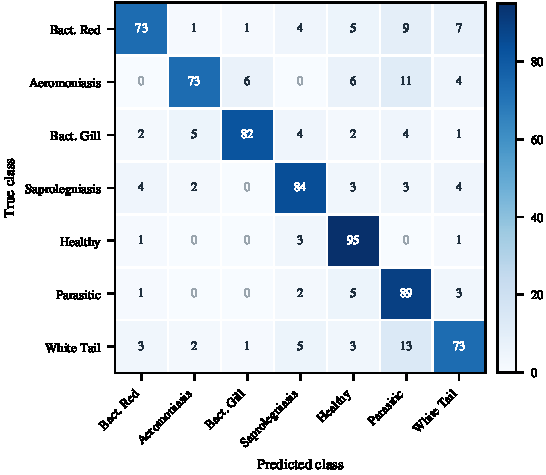
\includegraphics[width=0.62\columnwidth]{fig_confusion.pdf}
\caption{Confusion matrix on the 700-image test directory; rows are true classes, columns predicted. The dominant off-diagonal mass is the column under \emph{parasitic}, which absorbs 40 of the 131 errors.}
\label{fig:confusion}
\end{figure}

\emph{Parasitic disease behaves as an attractor.} Its column collects 40 misclassifications from the other six classes --- 13 from viral white tail, 11 from aeromoniasis, 9 from bacterial red --- which is 31\% of all errors and the widest bar in Fig.~\ref{fig:errorflow}. That is why its recall of 0.89 sits alongside a precision of 0.69, the lowest in the model. The cause is a lopsided decision boundary, not a shortage of examples: parasitic is where the network goes when it is unsure, and going there is cheap. Visible infestation shows up as small, scattered, locally high-contrast marks, and both haemorrhagic spotting and early white-tail lesions produce the same low-level signature. At $150\times150$ input the texture-scale cues that would separate them have already been resampled away.

\emph{Viral white tail disease is the weakest class} ($F_1=0.756$), losing 13 images to parasitic and 5 to fungal saprolegniasis. The fungal confusion at least makes sense on inspection: both present as pale discoloration of the caudal region, and telling a white lesion from a white fungal mat is a fine-texture call that survives neither the resize nor the brightness jitter we apply during training.

\emph{The two non-gill bacterial classes are under-predicted symmetrically}, both at recall 0.73 against precision near 0.87, with errors scattering widely rather than concentrating on each other. This differs from \cite{b1}, where gill-versus-red confusion dominated: here bacterial gill disease is the strongest bacterial class ($F_1=0.863$), plausibly because gill pathology is localised to a consistent anatomical region and is therefore learnable as a position-anchored feature, whereas the other bacterial lesions may appear anywhere on the body.

\emph{Healthy fish is over-predicted}: recall 0.95 against precision 0.798, which means 24 diseased fish get labelled healthy. We regard this as the most damaging error in the matrix. A wrong disease name invites a second opinion; a false clean bill of health ends the investigation. The likely mechanism is mild or early presentation, where the lesion covers a small fraction of the frame and the image sits nearer the healthy manifold than its own class centroid.

Two caveats bound all of this. Every evaluation image was present during fitting, so these 131 are cases the network cannot reproduce even on data it has seen; on genuinely novel photographs the error set will be larger and probably shaped differently. And since one exact duplicate group and five near-duplicate pairs carry contradictory labels, a handful of these errors cannot be won at all. Going further than description --- actually attributing the patterns --- needs evidence the current artefacts do not hold: saved probability vectors, gradient attribution \cite{b30}, and per-image capture metadata.

\begin{figure}[!t]
\centering
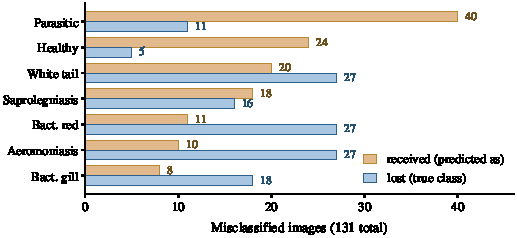
\includegraphics[width=\columnwidth]{fig_errorflow.pdf}
\caption{Where the 131 errors go. For each class, the blue bar counts images of that true class assigned elsewhere and the amber bar counts images of other classes assigned to it. Parasitic disease receives almost four times as many errors as it loses; healthy fish shows the same asymmetry, which is the more dangerous of the two.}
\label{fig:errorflow}
\end{figure}

% =========================================================
% IV. APPLICATION
% =========================================================
\section{Application}
\label{sec:app}

\subsection{Service and Two-Stage Prediction Pipeline}
\label{subsec:service}

The backend is a FastAPI application \cite{b15} served by Uvicorn, exposing \texttt{GET /health}, \texttt{GET /model/info}, \texttt{GET /diseases}, and \texttt{POST /predict} alongside the assistant routes of Section~\ref{sec:llm}; every request is timed and the elapsed milliseconds returned in a response header, which is what lets the client display a per-scan latency figure. Model loading is layered so that the application degrades instead of failing outright: the service prefers a project-level Keras \texttt{.h5} artefact, falls back to a bundled copy, and finally to ONNX. Whichever one loads, its output width is checked against \texttt{labels.json} at startup, and a mismatch aborts the load rather than quietly serving mislabelled predictions. No inference path makes a network request; the deployed artefacts are a 25.3\,MB Keras file, an 8.4\,MB ONNX fallback, a 1.5\,kB label map, and a 4.7\,kB disease record file. Transport validation rejects empty bodies and uploads above 15\,MB and checks content types against an allowlist.

\subsubsection{Fish-presence gate}
\label{subsec:gate}

A closed seven-way classifier will assign a disease to any input \cite{b25}. To prevent this, an ImageNet-pretrained \cite{b26} MobileNetV2 \cite{b7} is run first on a $224\times224$ resize of the same image. Let $\mathbf{p}\in\Delta^{999}$ be its 1000-way output and $\mathcal{F}$ the set of 16 ImageNet indices corresponding to fish --- tench, goldfish, great white shark, tiger shark, hammerhead, electric ray, stingray, barracouta, eel, coho, rock beauty, anemone fish, sturgeon, gar, lionfish, and puffer. The gate computes an aggregate fish score $s_{\mathrm{fish}}=\sum_{c\in\mathcal{F}}p_c$ and admits the image when

\begin{equation}
\arg\max_{c} p_c \in \mathcal{F}
\quad\text{or}\quad
s_{\mathrm{fish}} \;\geq\; \tau_g ,
\qquad \tau_g = 0.05 .
\label{eq:gate}
\end{equation}

The disjunction is doing real work. Farmed carp and tilapia are not ImageNet categories, so a diseased carp usually spreads modest probability over several fish classes without any single one winning; the aggregate term catches that case, and the $\arg\max$ term catches the unambiguous fish that the aggregate would also admit. The threshold sits three orders of magnitude above the $1/1000$ chance level and is environment-configurable. The gate fails open --- if it cannot be loaded, the detector returns ``fish present'' with an availability flag cleared and the request proceeds --- so a malfunction never blocks a legitimate scan, at the cost that unavailability silently removes the protection; the gate is therefore warmed at startup and its status reported by \texttt{/health}. On rejection the response names the closest ImageNet label. We report no accuracy for the gate: measuring it requires a labelled fish/non-fish set that this project does not contain, and the protocol is given in Section~\ref{sec:future}.

\subsubsection{Uncertainty rejection and confidence tiering}
\label{subsec:confidence}

Let $\mathbf{q}\in\Delta^{6}$ be the seven-way softmax output and $H(\mathbf{q})=-\sum_k q_k\log q_k$ its Shannon entropy \cite{b24}, bounded above by $\log 7\approx1.9459$. The service declares ``No Fish Detected'' when

\begin{equation}
\max_k q_k < \tau_c
\quad\text{and}\quad
H(\mathbf{q}) > \tau_H ,
\qquad \tau_c = 0.20,\ \tau_H = 1.90 .
\label{eq:reject}
\end{equation}

The conjunction is deliberate, and we arrived at it the hard way. A maximum-probability test on its own \cite{b25} rejects far too much: chance level for seven classes is $1/7\approx0.143$, and phone photographs taken in bad light routinely produce a \emph{correct} top class at 0.30--0.45. That is a usable differential, not a failure, and throwing it away frustrates the user for no benefit. Requiring the distribution to be simultaneously low-confidence and near-uniform restricts rejection to outputs carrying essentially no signal --- $\tau_H=1.90$ is 97.6\% of maximum attainable entropy. Surviving predictions are labelled high ($\geq0.70$), medium ($\geq0.45$), or low confidence, with recommendation text generated per tier: high gives the treatment record directly, medium asks for a confirming photograph from another angle, and low states explicitly that the result is a hint and not a diagnosis. Because softmax outputs are known to be poorly calibrated \cite{b23}, these thresholds are interface operating points rather than calibrated posteriors. The response also carries the top-3 ranked classes with probabilities, elapsed inference time, the active backend, and any image-quality warning.

\subsection{Mobile Application}
\label{subsec:mobile}

The client is a Flutter application \cite{b14} (Dart SDK $\geq$ 3.3, Material 3) built from one codebase for Android, iOS, Windows, and the web. Fig.~\ref{fig:screens} shows it running on an Android handset. Capture goes through \texttt{image\_picker} with runtime permission handling at quality 90 and a maximum width of 1500\,px, and a local decode before upload warns the user below a 200\,px short side, above a 3:1 aspect ratio, or below 15\,kB. Prediction is a multipart \texttt{POST /predict} with a 30\,s timeout. A status service polls \texttt{/health} every 15\,s across four states and disables the scan buttons when the backend is unreachable, which is better than letting a scan fail after the photograph has already been taken. Alongside this the client offers an offline disease library, session-scoped scan history, optional Firebase Google Sign-In with a persistent guest mode, and the assistant panel of Section~\ref{sec:llm}.

\begin{figure*}[!t]
\centering
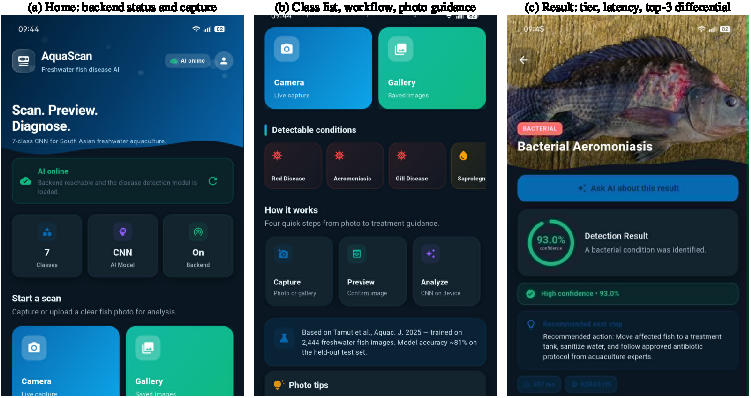
\includegraphics[width=0.70\textwidth]{fig_screens.pdf}
\caption{AquaScan on Android. (a) The home screen surfaces backend reachability before the user commits to a photograph. (b) Detectable conditions, the four-step workflow, and capture guidance. (c) A completed scan: confidence ring and tier badge, the tier-dependent recommendation, chips reporting 407\,ms of inference on the Keras backend, and the ranked top-3 differential (93.0\%, 4.9\%, 1.3\%).}
\label{fig:screens}
\end{figure*}

Two decisions in this client come from measured model behaviour rather than interface convention. The first is that the result screen shows a differential rather than a verdict: top-3 accuracy beats top-1 by 13.9 points, so the second and third ranked classes carry information worth showing, and Fig.~\ref{fig:screens}(c) presents all three with proportional bars. The second is that confidence is displayed, tiered, and acted on. The ring, the badge, and the recommendation text all read from the same thresholds the server uses, so a medium-confidence result looks like one everywhere in the interface. Given that the model over-predicts healthy fish (Section~\ref{subsec:error}), hiding uncertainty in the presentation layer would do active harm.

One inconsistency is worth naming rather than cropping out. The in-app copy visible in Fig.~\ref{fig:screens}(b) still describes 81\% as accuracy on a held-out test set, which is the framing we used before the audit of Section~\ref{subsec:dataset}. Correcting that string, and reporting the internal-validation figure instead, is part of the deployment work in Section~\ref{sec:future}. The backend is covered by four \texttt{pytest} suites exercising upload validation, health and model metadata, label-map consistency, top-3 ordering, prediction determinism for identical input bytes, and preprocessing parity, and the client carries unit and widget tests for authentication, the prediction service, the assistant controller, and application boot.

% =========================================================
% V. LLM INTEGRATION
% =========================================================
\section{LLM Integration}
\label{sec:llm}

A disease label answers one question and immediately raises four more. What causes this? How does it spread? What water conditions favour it? What should I do first? AquaScan handles those with a retrieval-augmented assistant \cite{b4} that runs entirely on the operator's machine (Fig.~\ref{fig:rag}).

\begin{figure*}[!t]
\centering
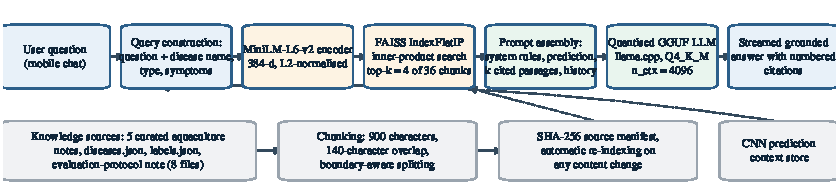
\includegraphics[width=0.74\textwidth]{fig_rag.pdf}
\caption{Retrieval-augmented assistant. The retrieval query concatenates the question with the current classifier output, so a follow-up is resolved against the detected condition. All generation is local.}
\label{fig:rag}
\end{figure*}

\subsection{Knowledge Base, Embedding, and Retrieval}
\label{subsec:kb}

The corpus is deliberately small and curated rather than scraped: five hand-written aquaculture notes covering biosecurity, common conditions and differentials, interpretation of model predictions, species and feeding, and water quality (1\,913 words in total), plus the application's structured disease record file, the canonical label map, and the project's evaluation protocol note. Structured sources are linearised into field/value prose before indexing, so a disease record becomes a paragraph rather than a JSON fragment, and the ingestion layer also accepts CSV, PDF, and Excel --- the path by which farm-specific guidance would be added. Documents are split into 900-character chunks with 140-character overlap at paragraph, sentence, or word boundaries, yielding 36 chunks. Index freshness is managed by content: a manifest records the SHA-256 digest, size, and modification time of every source together with the embedding model and chunking parameters, and any difference triggers an automatic atomic rebuild.

Chunks are embedded with \texttt{all-MiniLM-L6-v2} \cite{b5}, \cite{b37} into 384-dimensional $\ell_2$-normalised vectors and stored in a FAISS \texttt{IndexFlatIP} index \cite{b6}. With normalised vectors, inner product is cosine similarity, and at 36 chunks an exact flat index is both faster and simpler than an approximate one --- the persisted index is 54\,kB. The encoder loads from a local cache; the only point at which the system may contact a network is the first-time download of these weights, after which it is fully offline.

Retrieval is conditioned on the classifier, which is the part of this design we consider load-bearing. Rather than embedding the question on its own, the retriever forms

\begin{equation}
\tilde{q} \;=\; q \,\oplus\, d_{\mathrm{name}} \,\oplus\, d_{\mathrm{type}}
\,\oplus\, d_{\mathrm{symptoms}} ,
\label{eq:query}
\end{equation}

where $q$ is the question and the remaining terms come from the prediction context attached to the session, and retrieves the top $k=4$ chunks by inner product. That is what makes ``how do I treat this?'' answerable at all: the pronoun gets grounded by the classifier output before the query ever reaches the index. With no prediction attached, $\tilde{q}$ collapses to $q$ and the assistant falls back to being a general aquaculture reference. Context enters the session automatically --- \texttt{/predict} accepts an optional session identifier and on success publishes the full prediction payload to that session's context store, with publication failures logged and swallowed so that an assistant fault can never fail a scan.

\subsection{Prompt Construction and Local Generation}
\label{subsec:generation}

The assembled prompt contains a system instruction, the current prediction serialised as JSON, the $k$ retrieved passages numbered \texttt{[1]}--\texttt{[k]} with titles and source paths, up to six turns of history, and the question. The system instruction encodes the project's clinical posture explicitly: retrieved documents are reference data and never instructions; useful passages must be cited by number; absent or conflicting evidence must be stated rather than filled in; a softmax score is a model probability and not clinical certainty \cite{b23}; the assistant must not claim to know which image regions drove a prediction; ``No Fish Detected'' and low-confidence outputs are not diagnoses; antibiotic dosing is never prescribed, because it depends on jurisdiction, species, and withdrawal period; and professional confirmation is recommended before medication or culling. The assistant is an information tool, not a diagnostic authority.

Generation runs through \texttt{llama.cpp} \cite{b13} on quantised GGUF weights, with three models switchable at runtime --- Qwen3-8B (default), Mistral-7B-Instruct-v0.2, and Llama-3.1-8B-Instruct --- each at \texttt{Q4\_K\_M} quantisation and 4.1--4.7\,GiB on disk. Prompts are rendered with the native control tokens and stop sequences of each family rather than a generic template, and reasoning spans emitted by the Qwen model are stripped by a state machine that tolerates tags split across token boundaries. Decoding uses a 4096-token context, a 256-token output cap, temperature 0.35, top-$p$ 0.90, top-$k$ 40, and repetition penalty 1.12, with prompt length checked against the context window beforehand so that an overlong conversation produces an actionable error rather than a truncation. A low-memory mode keeps quantised weights memory-mapped instead of repacked into committed RAM, which is what allows an 8B model to coexist with the TensorFlow inference process on a 16\,GB machine; one model is resident at a time and concurrent requests are refused rather than queued. Answers stream as newline-delimited JSON whose first event carries the model, the retrieved sources, and the active prediction, so provenance is displayed before the first token arrives, and conversations persist in a local SQLite database keyed by session. Three things separate this from a general-purpose chatbot. The answer is drawn from a corpus the operator controls and can extend. The passages behind it are shown next to it. And no image, prediction, or question ever leaves the machine.

Fig.~\ref{fig:assistant} shows one exchange in the deployed client. The header reports the active generator and the scan in context, and the reply carries \texttt{[1]} markers back to the retrieved passage. Two details are worth pointing out, both of which follow from the system instruction rather than from luck. The assistant states that it cannot identify the fish species from the image, which is correct --- species is not something the classifier predicts and not something the knowledge base contains --- rather than guessing a plausible name. And it presents the 93.0\% output as a model probability attached to a named condition, then moves on to differential diagnoses instead of closing the question. We show this as an illustration of the intended behaviour, not as evidence of it: one conversation is not a measurement, and Section~\ref{subsec:ragEval} sets out what a measurement would require.

\begin{figure}[!t]
\centering

\includegraphics[width=\columnwidth]{fig_assistant.pdf}
\caption{The assistant answering a follow-up question about the scan in Fig.~\ref{fig:screens}(c). The context bar names the prediction the retrieval query is conditioned on, \texttt{[1]} markers point back to retrieved passages, and the reply declines to name the fish species rather than inventing one.}
\label{fig:assistant}
\end{figure}

\subsection{Evaluation Protocol for the Assistant}
\label{subsec:ragEval}

We have not evaluated the retrieval or generation components, and we report no numbers for them. What we do have is functional coverage: automated tests verify the streaming contract, session validation, single-flight generation locking, history persistence, prediction-context publication, and index rebuild-on-change. Those establish that the pipeline behaves as specified. They say nothing whatsoever about whether the answers are any good.

The protocol we regard as necessary before any quality claim follows. \emph{Benchmark:} at least 120 aquaculture questions stratified across eight intents --- symptoms, causal agents, prevention, treatment and management, water quality, biosecurity, differential diagnosis between visually similar conditions, and interpretation of a model prediction --- each annotated by a domain expert with the chunks containing the answer and a reference answer, and including at least 20 questions whose answers are deliberately \emph{absent} from the corpus, since correct refusal is a measurable property the system instruction requires. \emph{Retrieval:} Recall@$k$ and Precision@$k$ for $k\in\{1,2,4,8\}$ against the expert annotations, plus mean reciprocal rank and nDCG \cite{b42}, where

\begin{equation}
\mathrm{Recall}@k = \frac{|\{\text{queries with a relevant chunk in top-}k\}|}
{|\{\text{queries}\}|} .
\label{eq:recall}
\end{equation}

The production setting $k=4$ over a 36-chunk index must be validated rather than assumed. \emph{Grounding:} each generated claim labelled supported, contradicted, or unsupported with respect to the retrieved passages, giving a grounding rate and an unsupported-claim rate, with citation correctness scored separately as the fraction of \texttt{[n]} markers pointing to a passage that actually contains the cited content --- a plausible answer with a wrong citation is a specific and serious failure. Automated approximations \cite{b40} may be used for iteration, but reported figures should rest on expert adjudication with inter-annotator agreement stated. \emph{Hallucination and safety:} hallucination frequency measured on the unanswerable subset as the rate at which the assistant answers rather than declining \cite{b41}, and adherence to the safety constraints scored as a separate pass rate. \emph{Latency:} time to first token and total generation time, median and 95th percentile, per model and hardware, since a 4\,GiB quantised model on CPU is the binding usability constraint in the field. Until those measurements exist, the assistant is an implemented architecture of unmeasured quality, and we would rather say so than publish a plausible-looking score.

% =========================================================
% VI. FUTURE WORK
% =========================================================
\section{Future Work}
\label{sec:future}

The first four items validate claims already made and are ordered by how much they would change this paper's conclusions.

\textbf{A clean split, and the comparison that depends on it.} Nothing else on this list matters until the evaluation set can be trusted. Since the distributed test directory is a strict subset of the training directory, the partition must be rebuilt from the 1\,747 distinct images: collapse exact-duplicate groups to one representative, resolve or discard the pairs carrying conflicting labels, cluster near-duplicates at Hamming distance $\leq4$, and split at the level of groups rather than images. The partition should be published alongside the model so subsequent work is comparable. All figures in Section~\ref{subsec:eval} must then be recomputed, and we expect them to fall; the 63.71\% internal validation accuracy is the better prior. On that split the four baselines of Section~\ref{subsec:baselines} should be trained under the protocol specified there, testing in particular whether replacing the 2.10\,M-parameter dense projection with global average pooling recovers most of the benefit of a modern backbone at a fraction of its cost. Field collection should then extend the corpus with expert-verified pond-side photographs under grouped splitting, recording species, farm, device, lighting, and disease stage so that performance can be reported per stratum; active learning \cite{b32} would let reviewed misclassifications re-enter training.

\textbf{Quantitative gate and OOD evaluation.} The gate ships in the product and has never been measured. Evaluation needs at least 300 fish photographs spanning the seven classes, farmed species outside the ImageNet fish taxonomy, and adverse conditions (underwater, occluded, at distance, turbid water, held in hand, in a net), and at least 300 non-fish images from the categories the gate will actually meet --- pond surfaces, tanks, nets, buckets, feed, aeration equipment, people and hands, scenery, screens, and blank or blurred frames. The gate should then be characterised by precision, recall, specificity, false-positive and false-negative rate, and accuracy with 95\% intervals, and by an ROC over $\tau_g$ so that the 0.05 operating point is justified rather than asserted \cite{b25}. The two disjuncts of (\ref{eq:gate}) should be ablated separately, since our expectation that the $\arg\max$ term alone fails on farmed carp and tilapia is an untested design rationale. The error types are not symmetric --- a false negative costs a retake, whereas a false positive delivers a fabricated disease label with a confidence percentage attached --- and fail-open behaviour should additionally be measured as an availability rate under memory pressure.

\textbf{Formal RAG evaluation.} The benchmark and metric suite of Section~\ref{subsec:ragEval} should be built and run in full across all three configured generators under identical retrieval conditions and decoding parameters, with expert review conducted by aquaculture practitioners rather than by the system's authors. Three ablations matter: retrieval depth $k$; the prediction-conditioned query of (\ref{eq:query}) against question-only retrieval, which is the component that most distinguishes this assistant from a generic document chatbot; and a retrieval-disabled condition, since the central claim of the design is that retrieval reduces unsupported claims relative to a parametric-only baseline, and without that ablation the claim remains untested.

\textbf{Calibration, significance, and attributed error analysis.} The evaluation pipeline should persist per-image probability vectors, not only aggregate metrics. That single change replaces the bound of (\ref{eq:mcnemar}) with exact McNemar tests \cite{b16}, \cite{b18}, makes expected calibration error and multiclass Brier score \cite{b22}, \cite{b23} computable, and allows errors to be stratified by confidence. Calibration matters directly because the interface exposes confidence and tiers its recommendations on it: if temperature scaling improves reliability, the 0.70 and 0.45 boundaries should be re-derived from the calibrated distribution so that a stated confidence of 0.70 corresponds to roughly a 70\% empirical hit rate. Bootstrap resampling \cite{b19} should accompany every reported difference. The error patterns of Section~\ref{subsec:error} should then be attributed rather than inferred: Grad-CAM \cite{b30} would indicate whether the network attends to lesions or to background artefacts, and capture metadata would separate photographic causes from genuine ambiguity. Input resolution should be revisited directly, since the $150\times150$ input inherited from \cite{b1} is the most likely single cause of the parasitic/white-tail and white-tail/fungal confusions.

\textbf{Deployment.} On-device inference through TensorFlow Lite \cite{b31} or ONNX Runtime Mobile would remove the local-server requirement, with post-quantisation accuracy loss, latency, and memory footprint reported on low-cost Android hardware; a staged path is realistic --- quantised CNN inference first, retrieval second, generation last, since the language model dominates memory. Localisation of the interface and, harder, of the retrieval corpus into Nepali, Bengali, and Hindi is a precondition for use by the farmers this system targets, and cross-lingual retrieval quality must be verified rather than assumed. Optional consented geotagging would allow scans to be aggregated into regional outbreak maps, a capability no individual prediction can provide, noting that the current privacy posture --- nothing leaves the machine --- is itself worth preserving.

% =========================================================
% VII. CONCLUSION
% =========================================================
\section{Conclusion}

We set out to build a fish disease tool and ended up, along the way, having to re-read the benchmark it was built on. A 2.20\,M-parameter convolutional network trained under a shared preprocessing contract reaches 81.29\% top-1 and 95.14\% top-3 accuracy with macro $F_1$ 0.812 on the distributed test directory, improving on an earlier checkpoint by 11.86 accuracy points at a significance level bounded by $p\leq7.9\times10^{-6}$ without requiring the paired agreement table. A content audit showed that all 700 images in that directory are byte-identical copies of training images, leaving 1\,747 distinct photographs in a nominally 2\,450-file corpus, which constrains how the 81.29\% figure --- and every other figure published on this corpus --- may be interpreted, and makes the 63.71\% internal validation accuracy the honest generalisation estimate available here. The classifier runs behind an ImageNet fish-presence gate and a joint confidence--entropy rejection rule, so a photograph of a bucket returns ``No Fish Detected'' rather than a disease, and its output is presented as a tiered three-item differential justified by the 13.9-point gap between top-3 and top-1 accuracy, while a retrieval-augmented assistant conditioned on that output answers follow-up questions from cited local passages without contacting a network. We have been equally explicit about what we did not measure. Comparative baselines, gate accuracy, and retrieval and grounding quality appear here as protocols and as outstanding work, not as estimates. Given the duplication finding, rebuilding the evaluation split comes before all of them. On a corpus where the test set is a copy of the training set, a higher number is not a better model.

% =========================================================
% REFERENCES (generated from references.bib)
% =========================================================
\bibliographystyle{IEEEtran}
\bibliography{references}

\end{document}
